
%(BEGIN_QUESTION)
% Copyright 2012, Tony R. Kuphaldt, released under the Creative Commons Attribution License (v 1.0)
% This means you may do almost anything with this work of mine, so long as you give me proper credit

Skriv integraluttrykket som representeres av det skyggelagte området i dette diagrammet (forutsatt at hver horisontale og vertikale inndeling i diagrammet har trinnverdi 1). Integraluttrykket for dette området har en {\it positiv} verdi:

$$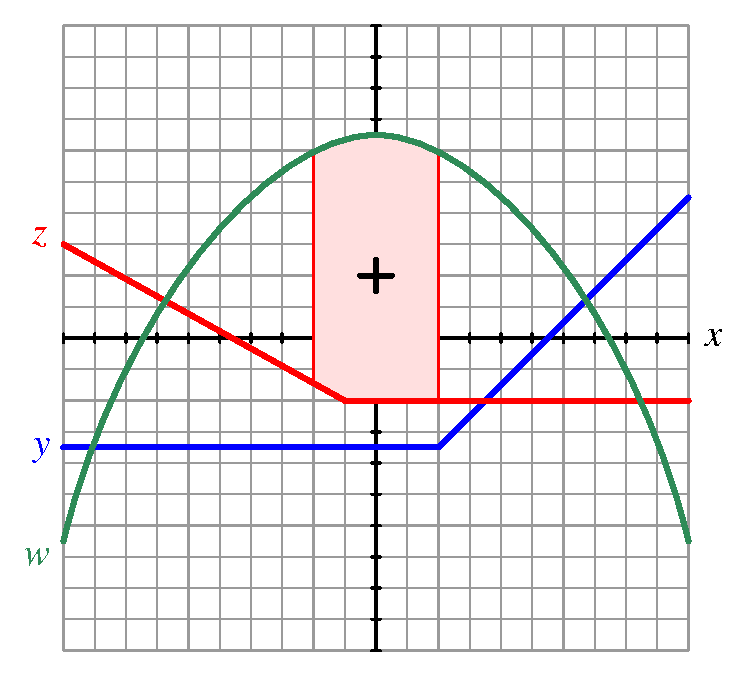
\includegraphics[width=15.5cm]{i01346x01.eps}$$

\underbar{file i01346}
%(END_QUESTION)





%(BEGIN_ANSWER)

Det finnes to ulike måter å skrive dette integralet på:

$$\int_{-2}^{2} (w - z) \> dx$$

$$\int_{2}^{-2} (z - w) \> dx$$

%(END_ANSWER)





%(BEGIN_NOTES)


%INDEX% Mathematics, calculus: integral (defined in a graphical sense)

%(END_NOTES)

